%-------------------------------------------------------------------------------
\section{Motivation}
%-------------------------------------------------------------------------------

Cloud providers like AWS, or containerization systems like Kubernetes, support
reserving CPU for \textit{latency critical} (LC) services. Developers choose
reservations based on expected peak load~\cite{borg, nu, overprovision}, but
load is variable, leading to a utilization problem. \textit{Best effort} (BE)
workloads do not have reservations, so providers run them opportunistically on
the same resources as LCs reserved; the resource that this work focuses on is
CPU. The challenge is to honor resource reservations for LCs while
opportunistically running BEs.

\begin{figure}[t]
    \centering
    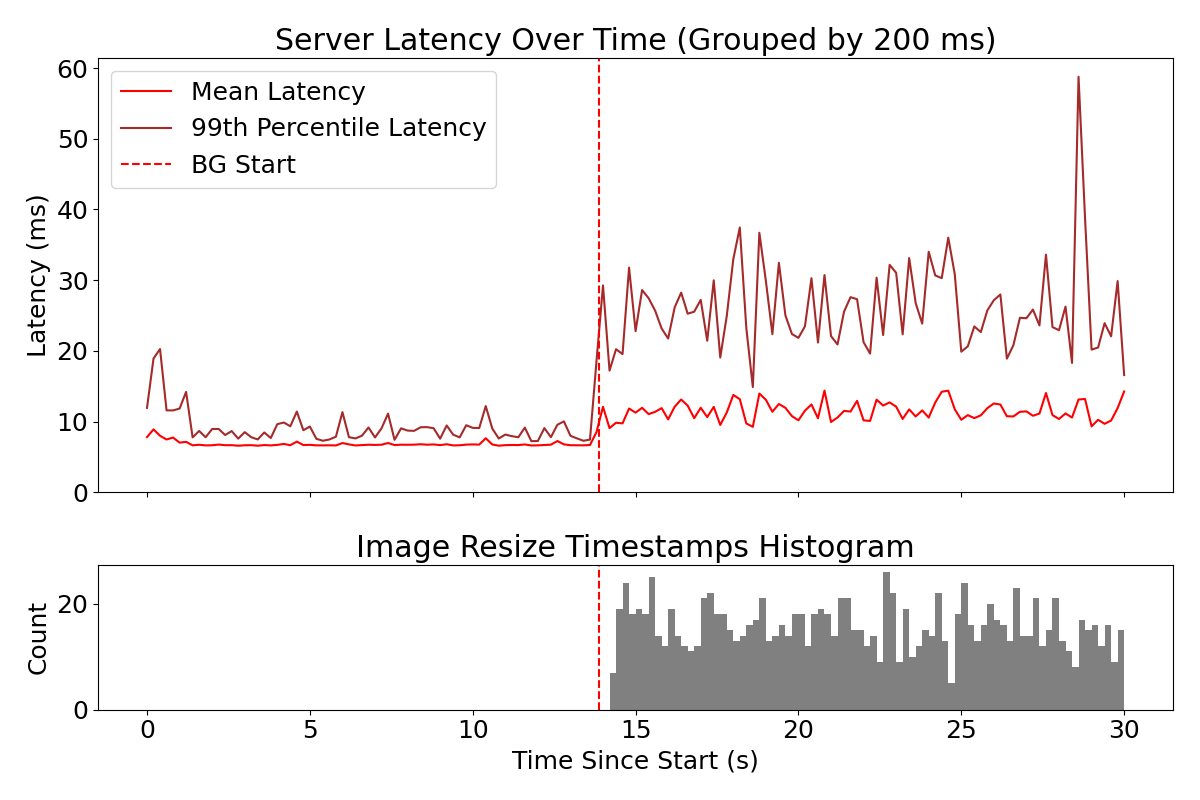
\includegraphics[width=\columnwidth]{graphs/kubernetes-unedited.png}
    \caption{In Kubernetes, running a BE has latency impacts on an LC with
    reservations}\label{fig:kubernetes-unedited}
\end{figure}
% In Kubernetes, running a BE has latency impacts on an LC with
%     reservations

Surprisingly, current popular scheduling systems fail to honor reservations.
$\autoref{fig:kubernetes-unedited}$ shows the latency of an endpoint in a web
application in Kubernetes that gets a user's feed, and the throughput of a BE
image resize job, both running on the same cores. The mean response latency
jumps from $\sim$7ms to $\sim$15ms after starting the BE.



